% Section 5 of motion_ctrl.tex (Layer-1 session, 2026-10-07): position-dependent motion gain, c-only slope law, q55 = 0.
%   Extension of Section 4 in the same layout; plane wall only (the unknown wall type and the meaning of c are Section 6).
%   Code: motion_control_law_formC_b.m via run_plaw_walls law 'f1p2' (slope (1-c)/h^2), production refinements ON and not
%   shown (user 10-07): y2 whitening, echo factor, MA(2), correlated n_x, and the d-step walk-back of y2 (the text writes the
%   delay-free H, measured harmless C92). c seeded at 0 (user 10-07), sqrt(P_cc[0]) = 0.1, q55 = 0, lambda_c 0.4.
%   Runs: test_script/scratch/run_mc_s5_conly.m (tags _mcs5_desc, _mcs5_tri); figures plot_mc_s5.m (first-order column =
%   run_mc_s4_first_order.m 'prod_xyz' / 'prod_tri10', same seed).
%   True gain step: the probe moves Delta x_d + (1-lc) dx3 + F_dx e_a + eps_x (from the tracking-error equation), so
%   a[k+1] = a + a'(M + F_dx e_a + eps_x); the eps_x part gives Q34 = -a' Q33, Q44 = a'^2 Q33 (formC_b header).
%   F_e row 4 = linearization at the estimate; written out (a)-(e) on its own page (user 10-07), from 0921_estb_v2_core.tex
%   section 6 (sympy: test_script/scratch/check_estb_v2_slope_c.py), in x-bar notation, without the L e[k] terms.
%   Update split (probe_mc_s5_update_split.m, 5 seeds, Fig. 5.2 plot_mc_s5_split.m): first order -- the prediction term is 0
%   (measured 1e-17), all of the change goes through l*e, sqrt(p44) 0.094 far / 0.053 near; c-only -- 99% of the near-wall drop
%   from a-hat' M-hat (-0.608 of -0.614), correction 1%; sqrt(p44) 0.0074 far / 0.023 near; rms correction per step 6.9e-3 vs
%   3.7e-5 far (185x), 4.5e-3 vs 1.1e-3 near.
%   Measured 10-07 (5 seeds, plane): descent end e_a c-only -0.025 (seed 1) vs first order -0.101; triangle 1.10-10 R 2 Hz:
%   troughs +0.004..+0.036 vs -0.06..-0.11, triangle mean |e_a| 0.039 vs 0.062, dz_m rms 0.029 vs 0.038 um; c-only tops sit
%   low (c_hat moves only near the wall); a_hat floor (0.05) hits 12 in 5 seeds -> dz_m spikes at some troughs.
\clearpage
\section{Real-time estimation with a position-dependent motion gain}

\hd{Motion gain as a function of the distance from the wall}
\[
\begin{aligned}
h[k] &= \bx_d[k] - \delta\bx_3[k] \\
\ba'[k] &= \frac{1 - c}{h[k]^{2}} \\
M[k] &= \Delta\bx_d[k] + (1-\lc)\,\delta\bx_3[k]
\end{aligned}
\]

\hd{State of the process}
\[
\begin{aligned}
\delta\bx_1[k+1] &= \delta\bx_2[k] \\
\delta\bx_2[k+1] &= \delta\bx_3[k] \\
\delta\bx_3[k+1] &= \lc\,\delta\bx_3[k] - F_{dx}[k]\,e_{\ba}[k] - \varepsilon_x[k] \\
\ba[k+1] &= \ba[k] + \ba'[k]\,\big(M[k] + F_{dx}[k]\,e_{\ba}[k] + \varepsilon_x[k]\big) \\
c[k+1] &= c[k]
\end{aligned}
\]

\hd{Measurement and output matrix}
\[
\mathbf{y}[k] = \begin{bmatrix} \delta\bx_m[k] \\ \ba_m[k] \end{bmatrix},
\qquad
\hat{\mathbf{y}}[k] = \begin{bmatrix} \delta\hat{\bx}_1[k] \\ \hat{\ba}[k] \end{bmatrix},
\qquad
\mathbf{H} =
\begin{bmatrix}
1 & 0 & 0 & 0 & 0 \\
0 & 0 & 0 & 1 & 0
\end{bmatrix}
\]

\hd{Estimator}
\[
\begin{aligned}
\hh[k] &= \bx_d[k] - \delta\hat{\bx}_3[k] \\
\hat{\ba}'[k] &= \frac{1 - \ch[k]}{\hh[k]^{2}} \\
\hat{M}[k] &= \Delta\bx_d[k] + (1-\lc)\,\delta\hat{\bx}_3[k]
\end{aligned}
\]
\[
\begin{aligned}
\delta\hat{\bx}_1[k+1] &= \delta\hat{\bx}_2[k] + \big\{\ell_{11}[k]\,e_{x_1}[k] + \ell_{12}[k]\,e_{a_m}[k]\big\} \\
\delta\hat{\bx}_2[k+1] &= \delta\hat{\bx}_3[k] + \big\{\ell_{21}[k]\,e_{x_1}[k] + \ell_{22}[k]\,e_{a_m}[k]\big\} \\
\delta\hat{\bx}_3[k+1] &= \lc\,\delta\hat{\bx}_3[k] + \big\{\ell_{31}[k]\,e_{x_1}[k] + \ell_{32}[k]\,e_{a_m}[k]\big\} \\
\hat{\ba}[k+1] &= \hat{\ba}[k] + \hat{\ba}'[k]\,\hat{M}[k] + \big\{\ell_{41}[k]\,e_{x_1}[k] + \ell_{42}[k]\,e_{a_m}[k]\big\} \\
\ch[k+1] &= \ch[k] + \big\{\ell_{51}[k]\,e_{x_1}[k] + \ell_{52}[k]\,e_{a_m}[k]\big\}
\end{aligned}
\]

\hd{Dynamics of estimation errors}
\[
\mathbf{e}[k] = \begin{bmatrix} e_{\delta\bx_1}[k] \\ e_{\delta\bx_2}[k] \\ e_{\delta\bx_3}[k] \\ e_{\ba}[k] \\ e_c[k] \end{bmatrix},
\qquad
\mathbf{e}[k+1] = \mathbf{F}_e[k]\,\mathbf{e}[k] - \mathbf{L}[k]\,\mathbf{H}\,\mathbf{e}[k] + \mathbf{q}[k]
\]
\[
\mathbf{F}_e[k] =
\begin{bmatrix}
0 & 1 & 0 & 0 & 0 \\
0 & 0 & 1 & 0 & 0 \\
0 & 0 & \lc & -F_{dx}[k] & 0 \\
0 & 0 & \;\hat{\ba}'[k]\,(1-\lc) + \dfrac{2\,\hat{\ba}'[k]}{\hh[k]}\,\hat{M}[k]\; & 1 + \hat{\ba}'[k]\,F_{dx}[k] & -\dfrac{\hat{M}[k]}{\hh[k]^{2}} \\
0 & 0 & 0 & 0 & 1
\end{bmatrix},
\qquad
\mathbf{q}[k] = \begin{bmatrix} 0 \\ 0 \\ -\varepsilon_x[k] \\ \hat{\ba}'[k]\,\varepsilon_x[k] \\ 0 \end{bmatrix}
\]

\clearpage
\hd{Row 4 of $\mathbf{F}_e$, expanded}

\noindent (a) the two gain steps and their difference
\[
\begin{aligned}
\ba[k+1] - \ba[k] &= \ba'[k]\,\big(M[k] + F_{dx}[k]\,e_{\ba}[k] + \varepsilon_x[k]\big) \\
\hat{\ba}[k+1] - \hat{\ba}[k] &= \hat{\ba}'[k]\,\hat{M}[k] \\
e_{\ba}[k+1] - e_{\ba}[k] &= \ba'[k]\,M[k] - \hat{\ba}'[k]\,\hat{M}[k] + \ba'[k]\,F_{dx}[k]\,e_{\ba}[k] + \ba'[k]\,\varepsilon_x[k]
\end{aligned}
\]

\noindent (b) each factor written as its estimate plus its error
\[
\begin{aligned}
h[k] &= \hh[k] - e_{\delta\bx_3}[k], \qquad c = \ch[k] + e_c[k] \\
\ba'[k] &= \frac{1 - \ch[k] - e_c[k]}{\big(\hh[k] - e_{\delta\bx_3}[k]\big)^{2}}
= \hat{\ba}'[k] + \frac{2\,\hat{\ba}'[k]}{\hh[k]}\,e_{\delta\bx_3}[k] - \frac{1}{\hh[k]^{2}}\,e_c[k] + O(e^{2}) \\
M[k] &= \hat{M}[k] + (1-\lc)\,e_{\delta\bx_3}[k]
\end{aligned}
\]

\noindent (c) the product difference, exact
\[
\ba'[k]\,M[k] - \hat{\ba}'[k]\,\hat{M}[k]
= \hat{\ba}'[k]\,\big(M[k] - \hat{M}[k]\big) + \big(\ba'[k] - \hat{\ba}'[k]\big)\,\hat{M}[k] + \big(\ba'[k] - \hat{\ba}'[k]\big)\big(M[k] - \hat{M}[k]\big)
\]

\noindent (d) every term after substituting (b)
\[
\begin{aligned}
e_{\ba}[k+1] - e_{\ba}[k]
&= \hat{\ba}'[k]\,(1-\lc)\,e_{\delta\bx_3}[k] \\
&\quad + \frac{2\,\hat{\ba}'[k]}{\hh[k]}\,\hat{M}[k]\,e_{\delta\bx_3}[k] - \frac{\hat{M}[k]}{\hh[k]^{2}}\,e_c[k] \\
&\quad + \hat{\ba}'[k]\,F_{dx}[k]\,e_{\ba}[k] + \hat{\ba}'[k]\,\varepsilon_x[k] \\
&\quad + \Big(\frac{2\,\hat{\ba}'[k]}{\hh[k]}\,e_{\delta\bx_3}[k] - \frac{e_c[k]}{\hh[k]^{2}}\Big)\Big((1-\lc)\,e_{\delta\bx_3}[k] + F_{dx}[k]\,e_{\ba}[k] + \varepsilon_x[k]\Big) + O(e^{2})
\end{aligned}
\]

\noindent (e) first-order terms collected by error
\[
e_{\ba}[k+1] = \Big(\hat{\ba}'[k]\,(1-\lc) + \frac{2\,\hat{\ba}'[k]}{\hh[k]}\,\hat{M}[k]\Big)\,e_{\delta\bx_3}[k]
+ \big(1 + \hat{\ba}'[k]\,F_{dx}[k]\big)\,e_{\ba}[k]
- \frac{\hat{M}[k]}{\hh[k]^{2}}\,e_c[k]
+ \hat{\ba}'[k]\,\varepsilon_x[k]
\]

\hd{Process noise and measurement noise}
\[
\begin{aligned}
\mathbf{Q}[k] &=
\begin{bmatrix}
0 & 0 & 0 & 0 & 0 \\
0 & 0 & 0 & 0 & 0 \\
0 & 0 & q_{33}[k] & -\hat{\ba}'[k]\,q_{33}[k] & 0 \\
0 & 0 & -\hat{\ba}'[k]\,q_{33}[k] & \hat{\ba}'[k]^{2}\,q_{33}[k] & 0 \\
0 & 0 & 0 & 0 & q_{55}
\end{bmatrix},
\qquad q_{55} = 0 \\
\mathbf{R}[k] &= \mathrm{diag}\big(r_1,\ r_2[k]\big)
\end{aligned}
\]
($q_{33}$, $r_1$, $r_2$, $\mathbf{L}$, $\mathbf{P}$, $\mathbf{P}^f$ as in Section 4.)

\figpage{Fig.~5.1\quad First order vs position-dependent motion gain: descent}{z axis; Section 2 trajectory; left: Section 4 estimator; right: this section, $q_{55} = 0$; plane wall, $\lc = 0.4$, seed 1}{fig_mc_s5_desc_s1.png}
\clearpage\subsection*{Fig.~5.2\quad Change of the motion-gain estimate in one step: prediction and correction}
\noindent{\small\textcolor[gray]{0.35}{z axis; run of Fig.~5.1; left: Section 4; right: this section; top: accumulated from $t = 0$; bottom: $|\ell_{41}|$, $|\ell_{42}|$ (50 ms mean, log axis); seed 1}}
\[
\begin{aligned}
\text{Section 4:}\quad \hat{\ba}[k+1] - \hat{\ba}[k] &= \ell_{41}[k]\,e_{x_1}[k] + \ell_{42}[k]\,e_{a_m}[k] \\
\text{this section:}\quad \hat{\ba}[k+1] - \hat{\ba}[k] &= \hat{\ba}'[k]\,\hat{M}[k] + \ell_{41}[k]\,e_{x_1}[k] + \ell_{42}[k]\,e_{a_m}[k]
\end{aligned}
\]
\begin{center}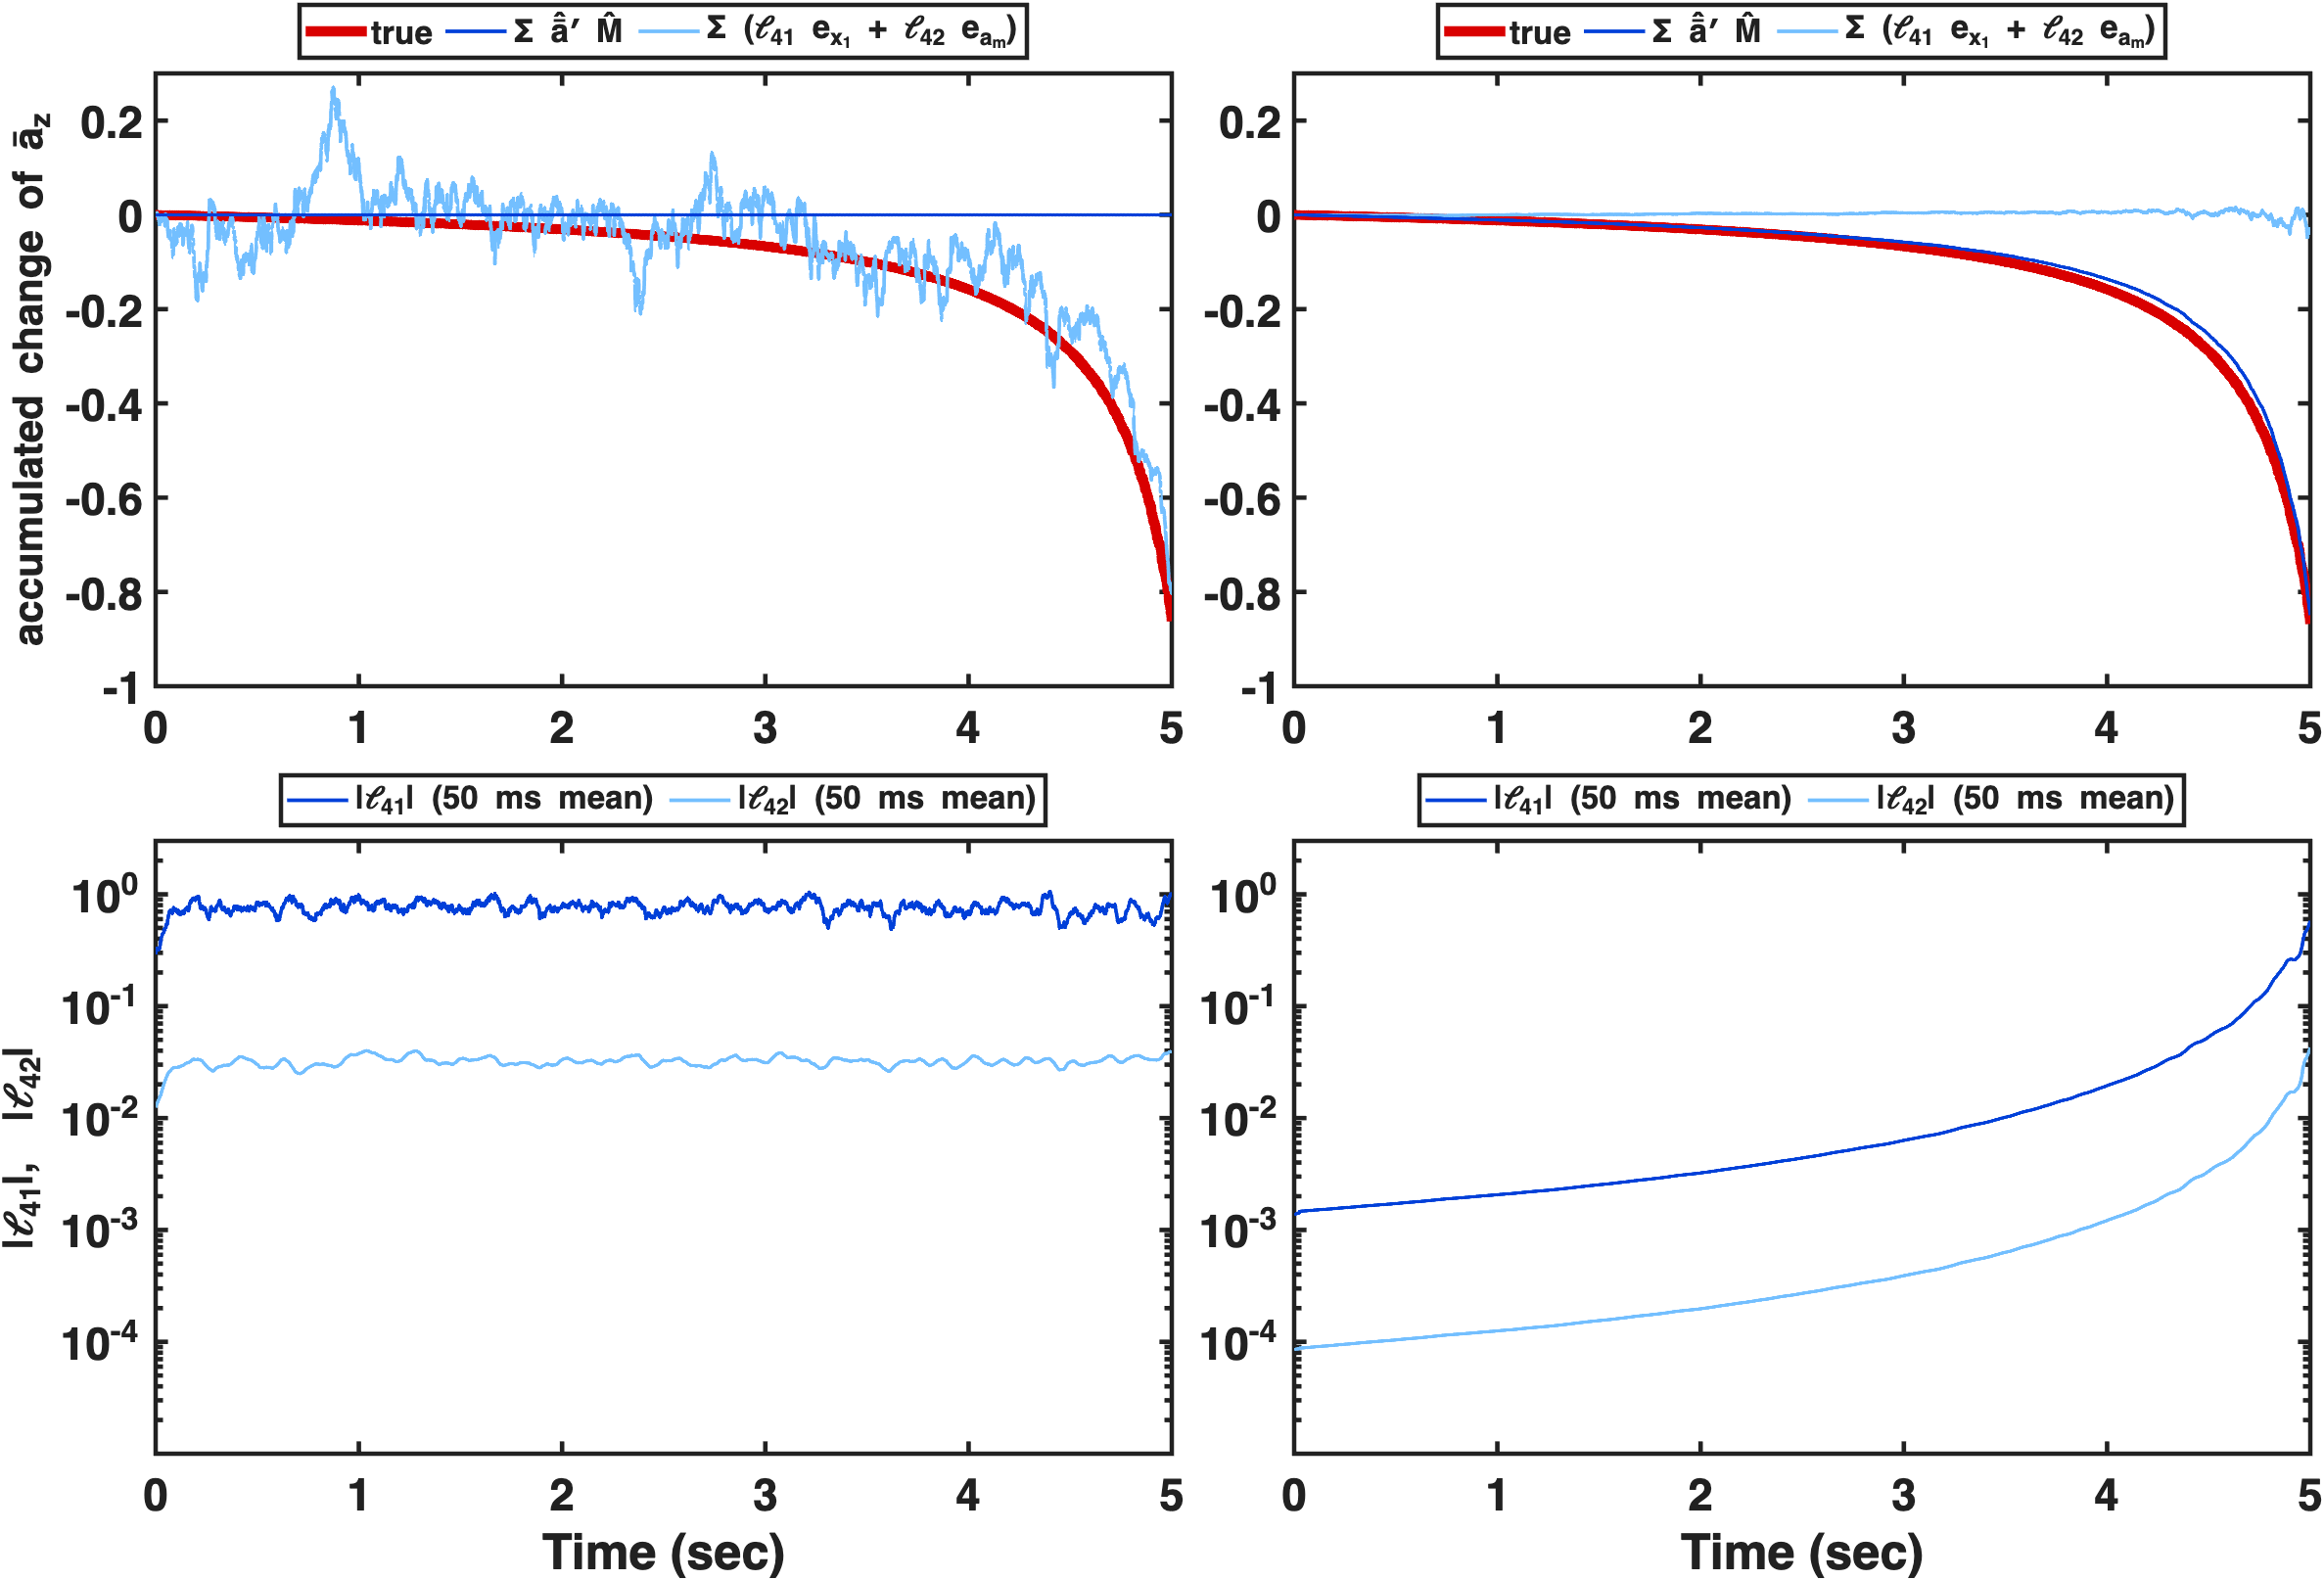
\includegraphics[width=\textwidth,height=0.68\textheight,keepaspectratio]{fig_mc_s5_split_s1.png}\end{center}
\figpage{Fig.~5.3\quad First order vs position-dependent motion gain: oscillation}{z axis; trajectory of Fig.~4.3 (triangle 1.10 $\leftrightarrow$ 10 R, 2 Hz); left: Section 4 estimator; right: this section, $q_{55} = 0$; plane wall, $\lc = 0.4$, seed 1}{fig_mc_s5_tri_s1.png}
